\documentclass[11pt,a4paper]{article}
\usepackage[utf8]{inputenc}
\usepackage[T1]{fontenc}
\usepackage{tgpagella}
\usepackage[spanish]{babel}
\usepackage{geometry}
\usepackage{booktabs}
\usepackage{xcolor}
\usepackage{titlesec}
\usepackage{fancyhdr}
\usepackage[parfill]{parskip}
\usepackage[expansion=false]{microtype}
\usepackage{hyperref}
\usepackage{setspace}
\usepackage{needspace}
\usepackage{graphicx}
\widowpenalty=10000
\clubpenalty=10000
\displaywidowpenalty=10000

\geometry{top=3.0cm,bottom=3.0cm,left=3.5cm,right=3.5cm}
\setlength{\parskip}{0.65em}
\setlength{\parindent}{0em}

\definecolor{azulai}{RGB}{30,80,140}
\definecolor{doradoai}{RGB}{140,90,0}
\definecolor{grisai}{RGB}{70,70,70}

\titleformat{\section}{\Large\bfseries\color{azulai}}{}{0em}{}[{\color{azulai}\titlerule[0.5pt]}]
\titlespacing*{\section}{0pt}{1.8em}{0.8em}
\titleformat{\subsection}{\large\bfseries\color{doradoai}}{}{0em}{}
\titlespacing*{\subsection}{0pt}{1.4em}{0.5em}
\titleformat{\subsubsection}{\normalsize\bfseries\color{grisai}}{}{0em}{}
\titlespacing*{\subsubsection}{0pt}{1.0em}{0.3em}

\pagestyle{fancy}\fancyhf{}
\rhead{\textcolor{grisai}{\small Maite Barragan — Arquitectura Interna}}
\lhead{\textcolor{grisai}{\small Júpiter · Saturno}}
\cfoot{\textcolor{grisai}{\small\thepage}}
\renewcommand{\headrulewidth}{0.3pt}

\hypersetup{colorlinks=true,linkcolor=azulai,urlcolor=azulai}
\setstretch{1.45}
\tolerance=1500
\emergencystretch=4em

\begin{document}

% ── Portada ──────────────────────────────────────────────────────────────────

\begin{titlepage}
\centering

\vspace*{2cm}

{\Huge\bfseries\color{azulai} Júpiter · Saturno}\\[0.4cm]

{\large\color{grisai} Arquitectura Interna}\\[0.25cm]

{\small\itshape\color{grisai}
Crecimiento, estructura y organización interna
}\\[1.8cm]

{\huge\color{doradoai} Maite Barragan}\\[1.2cm]

{\Large 07/01/1971 \quad 12:15}\\[0.25cm]

{\Large Pamplona, España}\\[0.25cm]

{\normalsize
Lat: 42.8157° \quad
Lon: -1.6522° \quad
UTC+01:00
}\\[0.4cm]

{\normalsize
Ascendente: Aries 6°18'
\quad
MC: Capricornio 3°11'
}\\[1.6cm]

\begin{tabular}{ll}
\textbf{Júpiter:} & Escorpio — Casa 8 28°47' \\
\textbf{Saturno:} & Tauro — Casa 1 15°48' (Retrógrado) \\
\end{tabular}

\vfill

{\small\color{grisai}
Generado el 20/05/2026
}

\end{titlepage}

	ableofcontents
space{0.8cm}

% ── Datos de referencia ──────────────────────────────────────────────────────

\section{Datos de referencia}

\begin{center}
\begin{tabular}{llll}
\toprule
\textbf{Punto} & \textbf{Signo} & \textbf{Casa} & \textbf{Posición} \\
\midrule

Júpiter &
Escorpio &
Casa 8 &
28°47' \\

Saturno (Retrógrado) &
Tauro &
Casa 1 &
15°48' \\

Sol &
Capricornio &
Casa 10 &
16°30' \\

Luna &
Tauro &
Casa 2 &
27°50' \\

Mercurio &
Sagitario &
Casa 9 &
27°51' \\

Venus &
Sagitario &
Casa 8 &
0°23' \\

Marte &
Escorpio &
Casa 8 &
20°09' \\

Ascendente &
Aries &
--- &
6°18' \\

Medio Cielo &
Capricornio &
--- &
3°11' \\

\bottomrule
\end{tabular}
\end{center}

\vspace{0.8cm}

\subsection*{Aspectos entre funciones}

\begin{center}
\begin{tabular}{lllll}
  \toprule
  \textbf{Planeta 1} & \textbf{Asp.} & \textbf{Planeta 2} & \textbf{Tipo} & \textbf{Orbe} \\
  \midrule
  Saturno & tri & Sol & Trígono & 0.7° \\
  Júpiter & opo & Luna & Oposición & 0.9° \\
  Júpiter & conj & Venus & Conjunción & 1.6° \\
  Saturno & opo & Marte & Oposición & 4.4° \\
  Júpiter & tri & Quirón & Trígono & 7.3° \\
  Júpiter & conj & Marte & Conjunción & 8.6° \\
  \bottomrule
\end{tabular}
\end{center}

\vspace{1cm}

\begin{center}
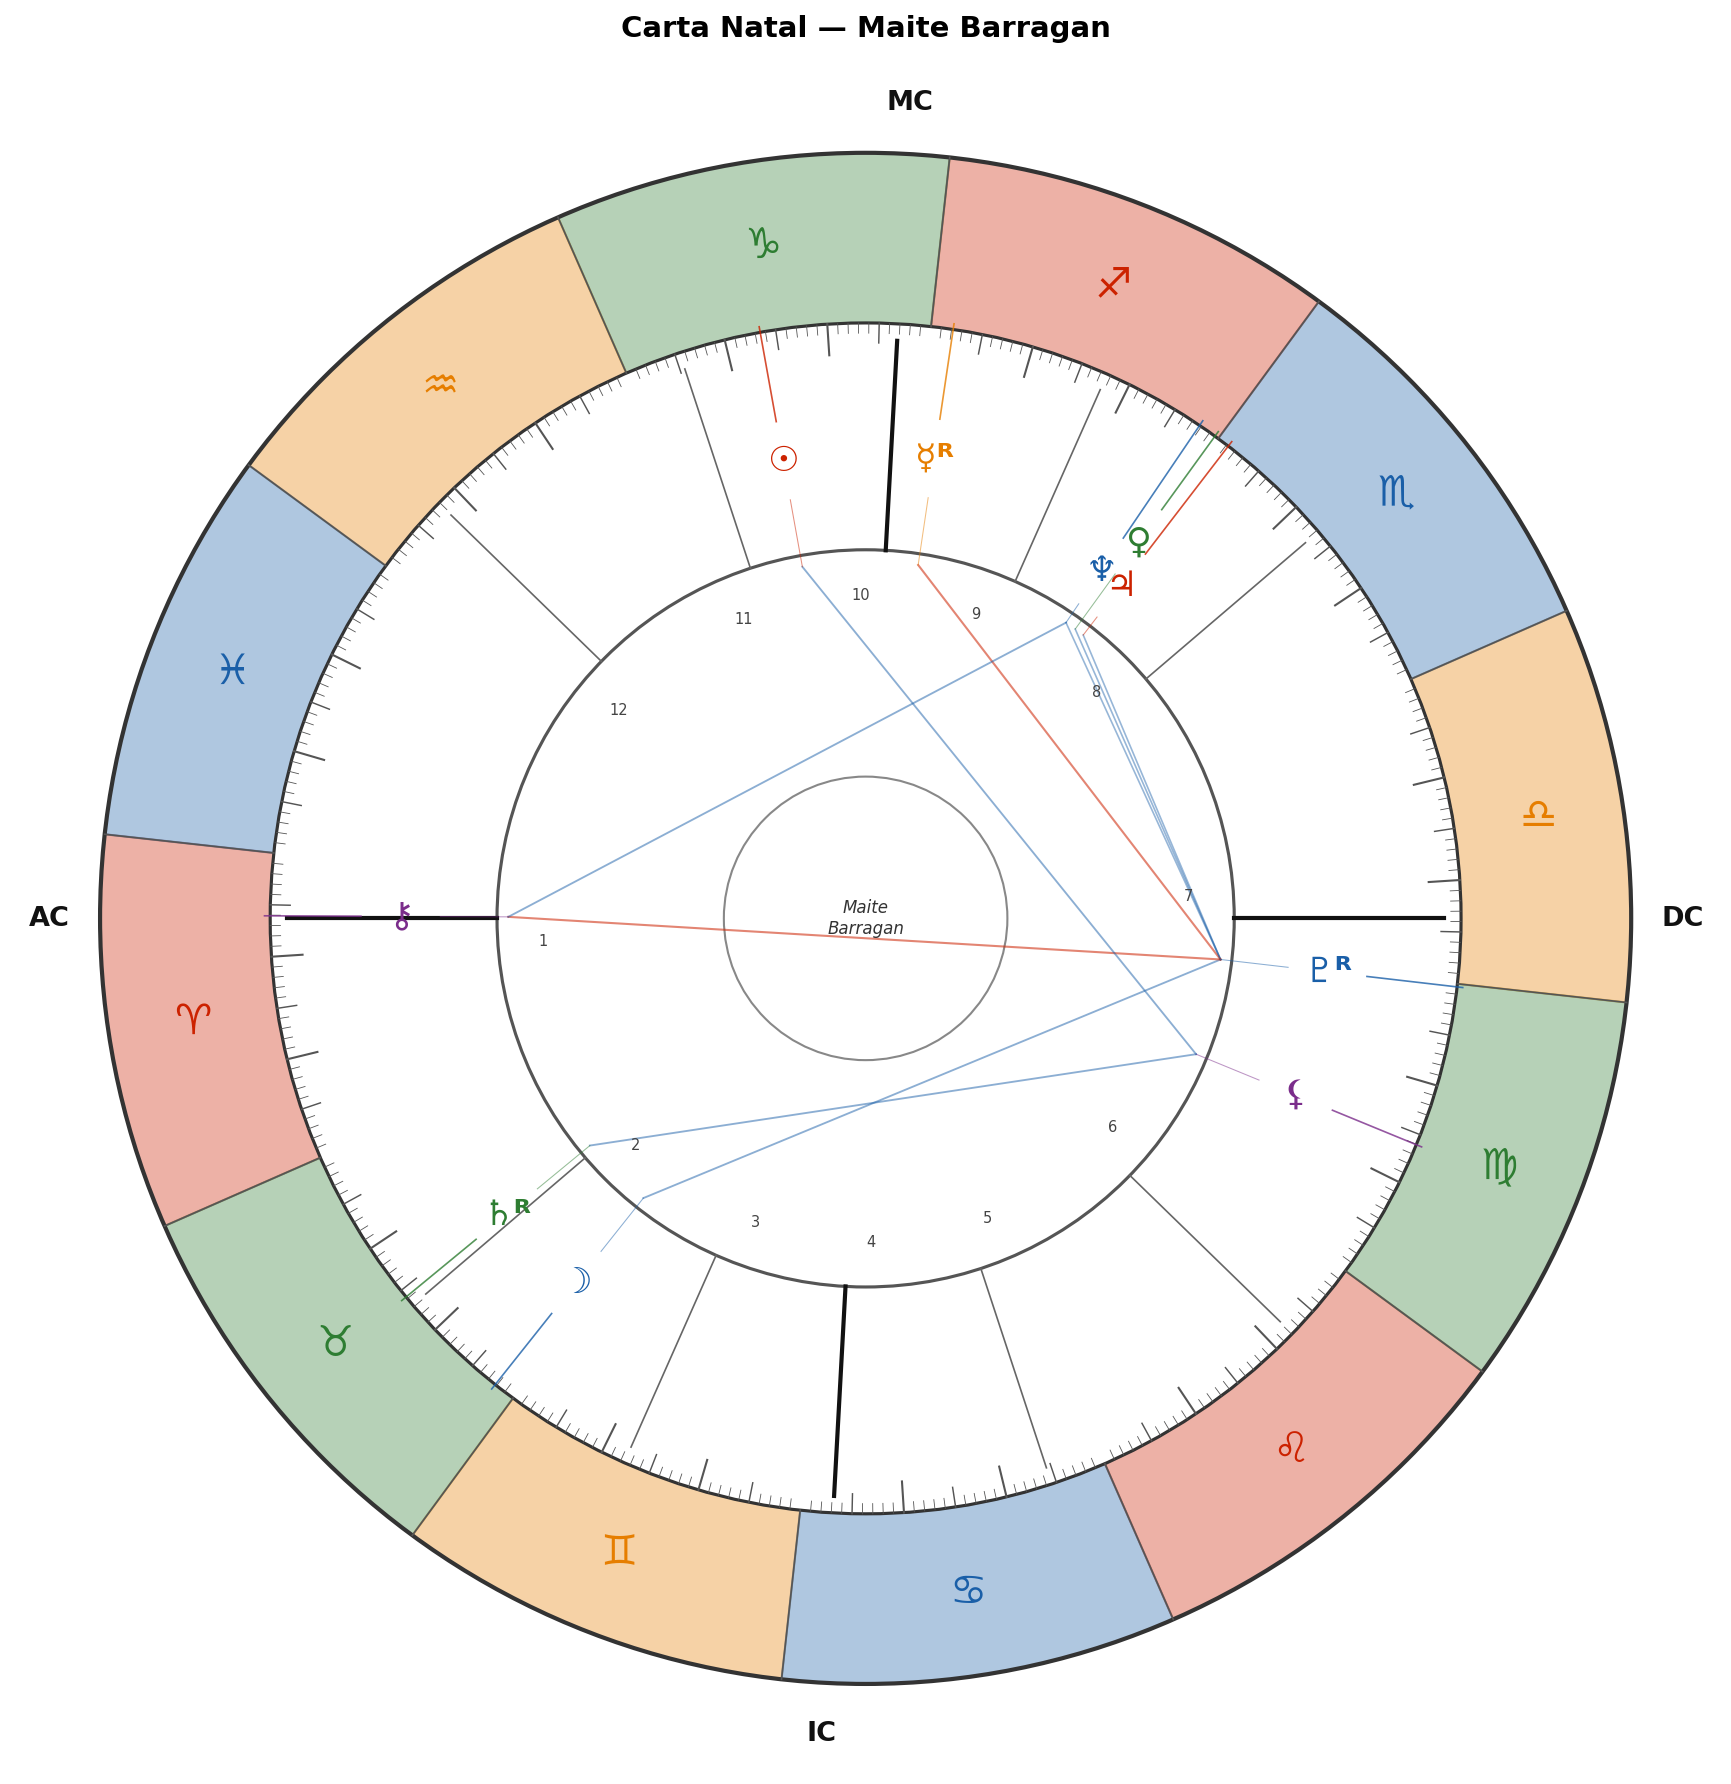
\includegraphics[width=0.72\textwidth]{Maite_Barragan_rueda.png}
\end{center}

\vspace{0.8cm}
\Needspace{5\baselineskip}


% ── Interpretación ───────────────────────────────────────────────────────────

\section{Interpretación — Arquitectura Interna}

\begin{center}
{\small\itshape
No se trata de definir quién eres.\\
Se trata de observar cómo tiendes a crecer, estructurarte\\
y sostener tu relación con el mundo.
}
\end{center}

\vspace{0.8cm}
\Needspace{5\baselineskip}

% ── 1. Estructura general ────────────────────────────────────────────────────

\subsection{1. Estructura general}

Júpiter está en Escorpio, Casa 8: muestra cómo tiendes a crecer, abrir posibilidades y ampliar tu relación con el mundo.
Saturno está en Tauro, Casa 1: muestra cómo tiendes a estructurarte, sostener límites y construir estabilidad.

Expansión (Escorpio, Agua) y estructura (Tauro, Tierra) operan en elementos compatibles. Esto puede facilitar que crecimiento y sostén colaboren con relativa naturalidad, aunque cada uno tenga un ritmo distinto.

Aspectos relevantes: Júpiter–Luna en oposición (orbe 0.95°), Júpiter–Venus en conjunción (orbe 1.6°), Júpiter–Marte en conjunción (orbe 8.63°), Saturno–Sol en trígono (orbe 0.71°), Saturno–Marte en oposición (orbe 4.36°).

\vspace{0.8cm}
\Needspace{5\baselineskip}

% ── 2. Júpiter ───────────────────────────────────────────────────────────────

\subsection{2. Júpiter — Expansión y crecimiento}

\subsubsection*{
Júpiter en Escorpio
— Casa 8
}

Tiendes a crecer a través de la profundidad, la transformación y el contacto con lo que no siempre es visible. La expansión aparece cuando puedes atravesar procesos intensos y comprender capas más profundas de la realidad o de ti misma. Necesitas sentir que lo que haces tiene densidad y verdad.

En situaciones de desbordamiento: la intensidad puede convertirse en control, invasión o exceso emocional. Puedes intentar profundizar más allá de lo que realmente puedes sostener. En momentos de estancamiento: la desconfianza dificulta abrirte a experiencias nuevas. La necesidad de protegerte termina limitando el crecimiento.

Tiendes a crecer atravesando procesos profundos de transformación y cambio. La expansión aparece cuando puedes entrar en contacto con capas menos visibles de la experiencia y desarrollar mayor profundidad emocional o psicológica. Necesitas intensidad, verdad y capacidad de atravesar procesos complejos.

Júpiter oposición Luna: expansión y regulación emocional tienden a competir entre sí. Cuando te abres a nuevas experiencias o posibilidades, puede costarte mantener estabilidad emocional. Cuando necesitas recogimiento o regulación, la expansión pierde fuerza.

Necesitas aprender a reconocer cuándo priorizar apertura y cuándo priorizar cuidado.

\vspace{0.8cm}
\Needspace{5\baselineskip}

% ── 3. Saturno ───────────────────────────────────────────────────────────────

\subsection{3. Saturno — Estructura y sostén}

\subsubsection*{
Saturno en Tauro
— Casa 1 (Retrógrado)
}

Tiendes a estructurarte construyendo estabilidad, continuidad y seguridad concreta. Necesitas tiempo para consolidar lo que haces y desarrollar una base sólida antes de abrir nuevos movimientos. La estructura suele fortalecerse lentamente, pero con mucha permanencia.

El límite aparece en la capacidad real de sostener lo acumulado. No todo lo que construyes puede mantenerse indefinidamente.

Cuando la estructura deja de sostenerse: puedes aferrarte a formas, vínculos o dinámicas que ya no funcionan. La necesidad de conservar estabilidad termina convirtiéndose en rigidez.

Tiendes a estructurarte a través de la presencia personal y la forma en que ocupas espacio en el mundo. La estabilidad se construye desarrollando una identidad coherente, sólida y capaz de sostenerse frente al entorno. Necesitas sentir consistencia entre quién eres, cómo actúas y cómo te presentas.

El límite aparece cuando intentas sostener una imagen o una forma de funcionar que ya no encaja contigo. No puedes separarte demasiado de tu propia estructura sin pagar un coste interno.

Saturno está retrógrado. La construcción de estructura suele desarrollarse de forma más interna y menos visible desde fuera al principio. Puedes necesitar tiempo antes de mostrar externamente algo que por dentro todavía estás consolidando.

Saturno trígono Sol: dirección y estructura colaboran con relativa estabilidad. Suele existir capacidad para sostener procesos largos, construir con coherencia y desarrollar algo de forma consistente.

\vspace{0.8cm}
\Needspace{5\baselineskip}

% ── 4. Integración ───────────────────────────────────────────────────────────

\subsection{4. Integración — Crecimiento y estructura}

Júpiter en Escorpio y Saturno en Tauro no forman aspecto directo y operan en elementos compatibles. La integración entre crecimiento y estructura tiene menor fricción de base. Precisamente por eso, conviene no asumir que se regulan solas: puedes entrar en sobreextensión o en rigidez progresiva sin detectarlo hasta que el coste ya es alto.

Cuando Júpiter domina: puedes absorber demasiado emocionalmente hasta perder la referencia de lo propio. La estructura de Saturno en Tauro no compensa con suficiente rapidez y lo que ganas en amplitud empieza a perder forma.

Cuando Saturno domina: puedes acumular tanta estructura que la forma termina impidiendo el movimiento. La expansión de Júpiter en Escorpio no encuentra espacio para activarse y puedes mantener lo que ya existe sin crecer hacia lo que sería posible.

Bajo presión suele aparecer una secuencia bastante reconocible. Primero, Saturno en Tauro empieza a ceder: pierdes estructura antes de haber construido una nueva base que la sustituya. Después, Júpiter en Escorpio ocupa ese espacio: absorbes demasiado de lo que ocurre alrededor sin poder procesarlo o diferenciarlo bien. Desde ahí puedes intentar recuperar estabilidad rápidamente, pero lo que construyes en ese estado suele ser más rígido, reactivo o agotador de sostener. Si el patrón no se reconoce a tiempo, el ciclo tiende a repetirse.

\vspace{0.8cm}
\Needspace{5\baselineskip}

% ── 5. Orientación práctica ──────────────────────────────────────────────────

\subsection{5. Orientación práctica}

\subsubsection*{Desde dónde empezar}

El punto de entrada más accesible suele estar en la estructura (Tauro, Casa 1). De las dos funciones, esta requiere menos resistencia para activarse. La forma más natural de empezar es llevar lo que ocurre a algo concreto, verificable y práctico. Cuando todo parece bloqueado, comenzar por aquí suele facilitar que la otra función también pueda ponerse en marcha.

\subsubsection*{Qué sostener}

Lo más importante de sostener aparece en Saturno (Tauro, Casa 1). Bajo presión puedes abrir posibilidades o reaccionar antes de mantener forma estable. Conviene cuidar especialmente mantener una estructura concreta aunque sea pequeña o sencilla. Muchas veces la primera señal de desgaste aparece cuando sigues haciendo cosas, pero ya no existe suficiente estructura para sostenerlas bien.

\subsubsection*{Qué evitar}

Conviene evitar asumir que la compatibilidad entre crecimiento y estructura garantiza integración automática. Cuando no existe fricción visible, ciertos desequilibrios pueden acumularse durante bastante tiempo antes de hacerse evidentes.

\subsubsection*{Si no se integra}

Cuando crecimiento y estructura dejan de colaborar, puede aparecer expansión sin suficiente sostén o estabilidad sin movimiento real. En ambos casos se pierde parte de lo que realmente podría desarrollarse si ambas funciones trabajaran en la misma dirección.

\subsubsection*{Señal temprana}

La primera señal suele aparecer en Saturno (Tauro): la acumulación empieza a superar la capacidad real de gestión. Cuando eso ocurre, Júpiter (Escorpio) tiende a ocupar rápidamente el espacio disponible y la expansión puede acelerarse más de lo que realmente puedes sostener. Detectar la señal temprano suele evitar entrar en ciclos más agotadores.

\vfill

\begin{center}
{\small\itshape\color{grisai}
La astrología se utiliza aquí como herramienta simbólica de observación\\
y no como una definición cerrada de la persona.
}
\end{center}

\end{document}
